\documentclass[a4paper,11pt]{article}
\input{/home/tof/Documents/Cozy/latex-include/preambule_doc.tex}
\input{/home/tof/Documents/Cozy/latex-include/preambule_commun.tex}
\newcommand{\showprof}{show them}  % comment this line if you don't want to see todo environment
\setlength{\fboxrule}{0.8pt}
\fancyhead[L]{\fbox{\Large{\textbf{ProgDyn 02}}}}
\fancyhead[C]{\textbf{Rendu de monnaie}}
\newdate{madate}{10}{09}{2020}
%\fancyhead[R]{\displaydate{madate}} %\today
%\fancyhead[R]{Seconde - SNT}
%\fancyhead[R]{Première - NSI}
\fancyhead[R]{Terminale - NSI}
\fancyfoot[L]{\vspace{1mm}Christophe Viroulaud}
\AtEndDocument{\label{lastpage}}
\fancyfoot[C]{\textbf{Page \thepage/\pageref{lastpage}}}
\fancyfoot[R]{\includegraphics[width=2cm,align=t]{/home/tof/Documents/Cozy/latex-include/cc.png}}
\usepackage{tikz}

\begin{document}
\section{Problématique}
L'approche gloutonne du rendu de monnaie permet de résoudre efficacement un problème qui a un temps de résolution long. Cependant la solution proposée peut dans certains cas de figure ne pas être optimale.
\begin{commentprof}
    problème NP-complet relativement à la taille du système monétaire. greedy algorithm = solution approchée
\end{commentprof}
\begin{center}
    \shadowbox{\parbox{13cm}{\centering Peut-on trouver une solution optimale en un temps raisonnable?}}
\end{center}
\section{Approche gloutonne}
\subsection{Algorithme}
Un algorithme glouton fait un choix sur lequel il ne revient pas.
\begin{center}
    \lstinputlisting[firstline=10 ,lastline= 19]{"scripts/rendu-monnaie.py"}
    \captionof{code}{Approche gloutonne}
    \label{glouton}
\end{center}

\subsection{Un exemple non optimal}
Choisissons un autre système de monnaie (code \ref{systeme}).
\begin{center}
    \begin{lstlisting}[language=Python]
    systeme = [30, 24, 12, 6, 3, 1]
    \end{lstlisting}
    \captionof{code}{Système monétaire impérial britannique}
    \label{systeme}
\end{center}
L'approche gloutonne ne donne pas la solution optimale.
\begin{activite}
    Dérouler à la main l'exécution de la fonction \emph{nb\_pieces\_glouton} pour 48€ avec le système (simplifié) de monnaie européenne puis le système impérial.
\end{activite}
\begin{aretenir}[Remarque]
    Le système monétaire européen est dit \emph{canonique}.
\end{aretenir}
\begin{commentprof}
    avant 1971, le système britannique n'était pas canonique: une livre sterling se divisait en 240 pence. Douze pence valaient un shilling et vingt shillings équivalaient à une livre.
\end{commentprof}
\section{Approche dynamique}
\subsection{Algorithme naïf}
Pour être certain de trouver la solution optimale il faut énumérer toutes les possibilités.
\begin{center}
    \lstinputlisting[firstline=33 ,lastline= 43]{"scripts/rendu-monnaie.py"}
    \captionof{code}{Approche naïve}
    \label{naif}
\end{center}
\begin{commentprof}
\begin{itemize}
    \item ligne 4 on initialise \emph{nb\_mini} pour avoir une référence
    \item tester toutes les solutions pour toutes les pièces du système (ligne 6)
    \item Je prends la pièce possible (1+ de la ligne 8) et je cherche toutes les solutions pour le reste à rendre
\end{itemize}
\end{commentprof}
\begin{center}
    \centering
    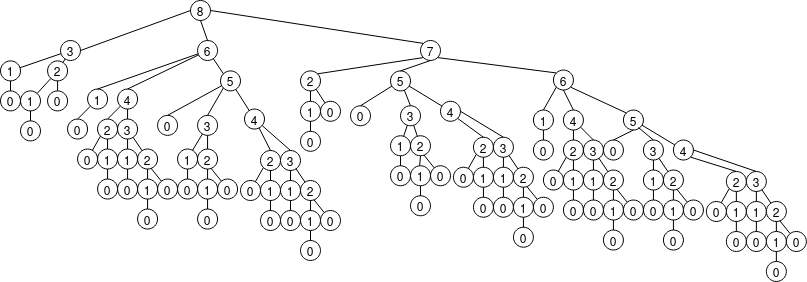
\includegraphics[width=17cm]{ressources/appel-naif-8.png}
    \captionof{figure}{Appels récursifs pour 8€}
    \label{IMG}
\end{center}
\begin{activite}
En s'aidant de l'arbre, dérouler l'exécution de la fonction (pour les premiers cas) à la main afin d'en comprendre le fonctionnement.
\end{activite}
\subsection{Top-down}
L'approche naïve montre une redondance dans les calculs. L'utilisation d'un tableau \emph{track} pour stocker les résultats intermédiaires permet d'éviter ce problème.
\begin{activite}
\begin{enumerate}
    \item Écrire la fonction \textbf{nb\_pieces\_TD(somme: int, systeme: list, track: list) $\;\rightarrow\;$int} qui reprend l'algorithme naïf et utilise le tableau \emph{track} de stockage intermédiaire.
    \item Tester la fonction pour les deux systèmes monétaires.
\end{enumerate}
\end{activite}
\begin{center}
    \centering
    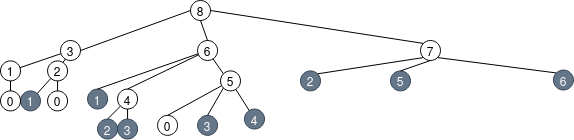
\includegraphics[width=17cm]{ressources/appel-dyn-8.png}
    \captionof{figure}{Approche dynamique pour 8€}
    \label{IMG}
\end{center}
\subsection{Bottom-up}
L'approche itérative \emph{bottom-up} trouve les solutions pour les petites sommes d'abord.
\begin{center}
    \lstinputlisting[firstline=77 ,lastline= 88]{"scripts/rendu-monnaie.py"}
    \captionof{code}{Approche bottom-up}
    \label{bu}
\end{center}
\begin{activite}
Écrire la fonction \textbf{nb\_pieces\_BU\_sol(somme: int, systeme: list) $\;\rightarrow\;$ list} qui renvoie la liste des pièces à choisir pour rendre la monnaie. On utilisera un tableau \emph{choix} de taille \emph{somme+1} où chaque élément de rang x contiendra la valeur de la première pièce à rendre pour la somme x.
\end{activite}
\end{document}